\documentclass{standalone}
\usepackage{tikz}
\usepackage{ctex,siunitx,ninecolors}
\usepackage{tkz-euclide}
\usepackage{amsmath}
\usetikzlibrary{patterns, calc}
\usetikzlibrary {decorations.pathmorphing, decorations.pathreplacing, decorations.shapes,}
\begin{document}
\small
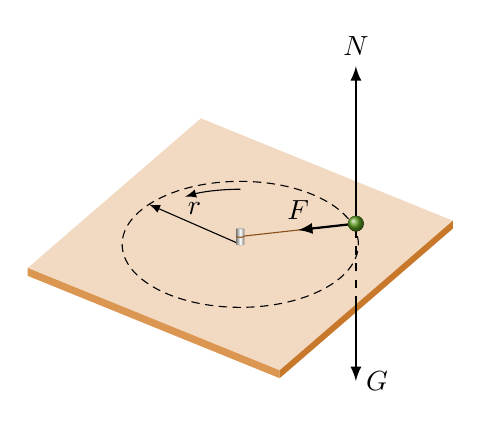
\begin{tikzpicture}[>=latex,scale=1]
  \fill[brown9](-2.7,-0.3)--(0.5,-1.6)--(2.7,0.3)--(-0.5,1.6);
  \fill[brown7](-2.7,-0.3)--(0.5,-1.6)--(0.5,-1.7)--(-2.7,-0.4);
  \fill[brown6](0.5,-1.6)--(0.5,-1.7)--(2.7,0.2)--(2.7,0.3);
  \draw[thin,->](0,0)--(-1.1597,0.5074)node[midway,above]{$r$};
  \draw[densely dashed](0,0)ellipse(1.5 and 0.8);
  \draw[brown4](0,0.1)--(1.4685,0.2632);
  \fill[left color=gray,right color=gray,middle color=white](-0.05,0)arc(180:360:0.05 and 0.01)--(0.05,0.2)--(-0.05,0.2)--cycle;
  \fill[lightgray](0,0.2)ellipse(0.05 and 0.01);
  \draw[brown4](-0.05,0.1)arc(180:360:0.05 and 0.01);
  \draw[thick,->](1.4685,0.2632)--++(0,2.0)node[above]{$N$};
  \draw[thick,dashed](1.4685,-0.7636)--(1.4685,0.2632);
  \draw[thick,->](1.4685,-0.7636)--(1.4685,-1.7368)node[right]{$G$};
  \draw[thick,->](1.4685,0.2632)--(0.7342,0.1816)node[above]{$F$};
  \fill[ball color=olive6](1.4685,0.2632)circle(0.1);
  \draw[thin,->](0,0.7)arc(90:120:1.4 and 0.7);
\end{tikzpicture}
\end{document}